\documentclass[12pt]{article}
\usepackage{amsthm,amssymb,amsfonts,amsmath,amstext,systeme}
\usepackage{graphicx,float}
\usepackage{tabularx}

\marginparwidth 0pt
\oddsidemargin -1.2 truecm
\evensidemargin  0pt 
\marginparsep 0pt
\topmargin -2.2truecm
\linespread{1}
\textheight 25.8 truecm
\textwidth 18.5 truecm
\newenvironment{remark}{\noindent{\bf Remark }}{\vspace{0mm}}
\newenvironment{remarks}{\noindent{\bf Remarks }}{\vspace{0mm}}
\newenvironment{question}{\noindent{\bf Question }}{\vspace{0mm}}
\newenvironment{questions}{\noindent{\bf Questions }}{\vspace{0mm}}
\newenvironment{note}{\noindent{\bf Note }}{\vspace{0mm}}
\newenvironment{summary}{\noindent{\bf Summary }}{\vspace{0mm}}
\newenvironment{back}{\noindent{\bf Background}}{\vspace{0mm}}
\newenvironment{conclude}{\noindent{\bf Conclusion}}{\vspace{0mm}}
\newenvironment{concludes}{\noindent{\bf Conclusions}}{\vspace{0mm}}
\newenvironment{dill}{\noindent{\bf Description of Dill's model}}{\vspace{0mm}}
\newenvironment{maths}{\noindent{\bf Mathematics needed}}{\vspace{0mm}}
\newenvironment{inst}{\noindent{\bf Instructions}}{\vspace{0mm}}
\newenvironment{notes}{\noindent{\bf Notes }}{\vspace{0mm}}
\newenvironment{theorem}{\noindent{\bf Theorem }}{\vspace{0mm}}
\newenvironment{example}{\noindent{\bf Example }}{\vspace{0mm}}
\newenvironment{examples}{\noindent{\bf Examples }}{\vspace{0mm}}
\newenvironment{topics}{\noindent{\bf Topics}}{\vspace{0mm}}
\newenvironment{outcomes}{\noindent{\bf Expected Learning Outcomes}}{\vspace{0mm}}
\newenvironment{lemma}{\noindent{\bf Lemma }}{\vspace{0mm}}
\newenvironment{solution}{\noindent{\it Solution}}{\vspace{2mm}}
\newcommand{\ds}{\displaystyle}
\newcommand{\un}{\underline}
\newcommand{\bs}{\boldsymbol}

\begin{document}

\baselineskip 18 pt
\begin{center}
	{\large \bf HKDSE MATH CORE 2018 Past Paper I}\\
	\vspace{2 mm}

\end{center}
\vspace{0.05cm}

\begin{enumerate}
	\item \textbf{HKDSE MATH CORE 2018 Past Paper I Q1}\\
	Make $b$ the subject of the formula $\dfrac{a+4}{3} = \dfrac{b+1}{2}$. \\(3 marks)

	\item \textbf{HKDSE MATH CORE 2018 Past Paper I Q2}\\
	Simplify $\dfrac{xy^7}{(x^{-2}y^3)^4}$ and express your answer with positive indices. \\(3 marks)

	\item \textbf{HKDSE MATH CORE 2018 Past Paper I Q3}
	\begin{enumerate}
		\item[(a)] Round up 265.473 to the nearest integer.
		\item[(b)] Round down 265.473 to 1 decimal place.
		\item[(c)] Round off 265.473 to 2 significant figures.
	\end{enumerate}
	(3 marks)

	\item \textbf{HKDSE MATH CORE 2018 Past Paper I Q4}\\
	A box contains $n$ white balls, 5 black balls and 8 red balls. If a ball is randomly drawn from the box, then the probability of drawing a red ball is $\dfrac{2}{5}$. Find the value of $n$. \\(3 marks)

	\item \textbf{HKDSE MATH CORE 2018 Past Paper I Q5}\\
	Factorize
	\begin{enumerate}
		\item[(a)] $9r^3 - 18r^2s$,
		\item[(b)] $9r^3 - 18r^2s - rs^2 + 2s^3$.
	\end{enumerate}
	(4 marks)

	\item \textbf{HKDSE MATH CORE 2018 Past Paper I Q6}
	\begin{enumerate}
		\item[(a)] Find the range of values of $x$ which satisfy both $\dfrac{3 - x}{2} > 2x + 7$ and $x + 8 \geq 0$.	   
		\item[(b)] Write down the greatest integer satisfying both inequalities in (a).	
	\end{enumerate}
	(4 marks)

	\item \textbf{HKDSE MATH CORE 2018 Past Paper I Q7}\\
	The marked price of a vase is 30\% above its cost. A loss of \$88 is made by selling the vase at a discount of 40\% on its marked price. Find the marked price of the vase. \\(5 marks)
	
	\item \textbf{HKDSE MATH CORE 2018 Past Paper I Q8}\\
	In Figure 1, $ABCDE$ is a circle. It is given that $AB // ED$. $AD$ and $BE$ intersect at the point $F$.
	\begin{figure}[H]
		\centering
		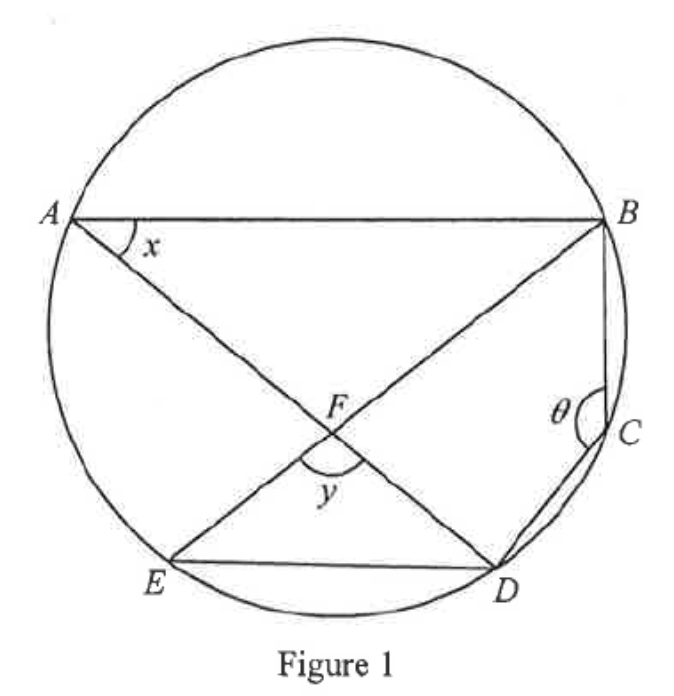
\includegraphics[width = .3\linewidth]{2018Figure1.1}
	\end{figure}
	Express $x$ and $y$ in terms of $\theta$. \\(5 marks)
	
	
	\item \textbf{HKDSE MATH CORE 2018 Past Paper I Q9}\\
	A car travels from city $P$ to city $Q$ at an average speed of 72 km/h and then the car travels from city $Q$ to city $R$ at an average speed of 90 km/h. It is given that the car travels 210 km in 161 minutes for the whole journey. How long does the car take to travel from city $P$ to city $Q$? \\(5 marks)

	\item \textbf{HKDSE MATH CORE 2018 Past Paper I Q10}\\
	The box-and-whisker diagram below shows the distribution of the ages of the clerks in team $X$ of a company. It is given that the range and the inter-quartile range of this distribution are 43 and 21 respectively.
	\begin{figure}[H]
		\centering
		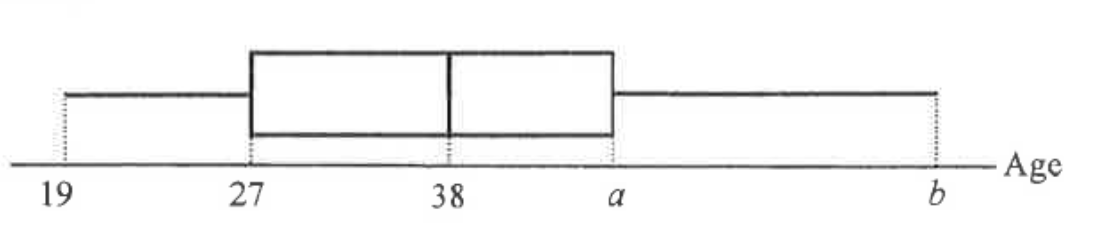
\includegraphics[width = .3\linewidth]{2018Figure1.00}
	\end{figure}
	\begin{enumerate}
		\item[(a)] Find $a$ and $b$. \\(3 marks)
		\item[(b)] There are five clerks in team $Y$ of the company and three of them are of age 38. It is given that the range of the ages in team $Y$ is 20. Team $X$ and team $Y$ are now combined to form a section. The manager of the company claims that the range of the ages of the clerks in the section and the range of the ages of the clerks in team $X$ must be the same. Do you agree? Explain your answer. \\(2 marks)
	\end{enumerate}

	\item \textbf{HKDSE MATH CORE 2018 Past Paper I Q11}\\
	The following table shows the distribution of the numbers of children of some families:
	$$\begin{array}{|c|c|c|c|c|c|}
		\hline
		\text{Number of children} & 0 & 1 & 2 & 3 & 4 \\
		\hline
		\text{Number of families} & k & 2 & 9 & 6 & 7 \\
		\hline
	\end{array}$$
	It is given that $k$ is a positive integer.
	\begin{enumerate}
		\item[(a)] If the mode of the distribution is 2, write down
		\begin{enumerate}
			\item[(i)] the least possible value of $k$;
			\item[(ii)] the greatest possible value of $k$.
		\end{enumerate}
		(2 marks)
		\item[(b)] If the median of the distribution is 2, write down
		\begin{enumerate}
			\item[(i)] the least possible value of $k$;
			\item[(ii)] the greatest possible value of $k$.
		\end{enumerate}
		(2 marks)
		\item[(c)] If the mean of the distribution is 2, find the value of $k$. \\(2 marks)
	\end{enumerate}

	\item \textbf{HKDSE MATH CORE 2018 Past Paper I Q12}\\
	Let $f(x) = 4x(x+1)^2 + ax + b$, where $a$ and $b$ are constants. It is given that $x - 3$ is a factor of $f(x)$. When $f(x)$ is divided by $x + 2$, the remainder is $2b + 165$.
	\begin{enumerate}
		\item[(a)] Find $a$ and $b$. \\(3 marks)
		\item[(b)] Someone claims that the equation $f(x) = 0$ has at least one irrational root. Do you agree? Explain your answer. \\(4 marks)
	\end{enumerate}

	\item \textbf{HKDSE MATH CORE 2018 Past Paper I Q13}\\
	In Figure 2, $ABCD$ is a trapezium with $\angle ABC = 90^\circ$ and $AB // DC$. $E$ is a point lying on $BC$ such that $\angle AED = 90^\circ$.
	\begin{figure}[H]
		\centering
		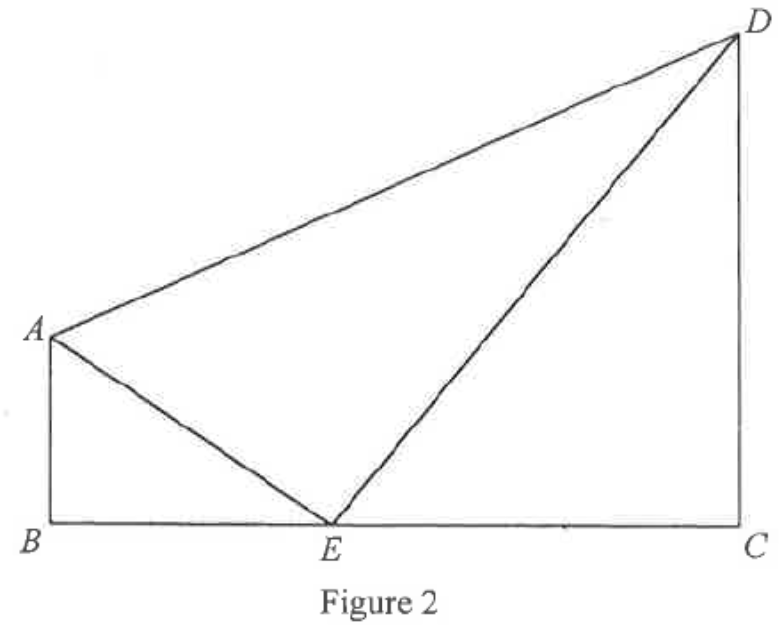
\includegraphics[width = .3\linewidth]{2018Figure1.2}
	\end{figure}
	\begin{enumerate}
		\item[(a)] Prove that $\triangle ABE \sim \triangle ECD$. \\(2 marks)
		\item[(b)] It is given that $AB = 15$ cm, $AE = 25$ cm and $CE = 36$ cm.
		\begin{enumerate}
			\item[(i)] Find the length of $CD$.
			\item[(ii)] Find the area of $\triangle ADE$.
			\item[(iii)] Is there a point $F$ lying on $AD$ such that the distance between $E$ and $F$ is less than 23 cm? Explain your answer.
		\end{enumerate}
		(6 marks)
	\end{enumerate}

	\item \textbf{HKDSE MATH CORE 2018 Past Paper I Q14}\\
	A right circular cylindrical container of base radius 8 cm and height 64 cm and an inverted right circular conical vessel of base radius 20 cm and height 60 cm are held vertically. The container is fully filled with water. The water in the container is now poured into the vessel.
	\begin{enumerate}
		\item[(a)] Find the volume of water in the vessel in terms of $\pi$. \\(2 marks)
		\item[(b)] Find the depth of water in the vessel. \\(4 marks)
		\item[(c)] If a solid meter sphere of radius 14 cm is then put into the vessel and the sphere is totally immersed in the water, will the water overflow? Explain your answer. \\(3 marks)
	\end{enumerate}

	\item \textbf{HKDSE MATH CORE 2018 Past Paper I Q15}\\
	An eight-digit phone number is formed by a permutation of 2, 3, 4, 5, 6, 7, 8 and 9.
	\begin{enumerate}
		\item[(a)] How many different eight-digit phone numbers can be formed? \\(1 mark)
		\item[(b)] If the first digit and the last digit of an eight-digit phone number are odd numbers, how many different eight-digit phone numbers can be formed? \\(2 marks)
	\end{enumerate}

	\item \textbf{HKDSE MATH CORE 2018 Past Paper I Q16}\\
	The 3rd term and the 4th term of a geometric sequence are 720 and 864 respectively.
	\begin{enumerate}
		\item[(a)] Find the 1st term of the sequence. \\(2 marks)
		\item[(b)] Find the greatest value of $n$ such that the sum of the $(n + 1)$th term and the $(2n + 1)$th term is less than $5 \time 10^{14}$. \\(3 marks)
	\end{enumerate}

	\item \textbf{HKDSE MATH CORE 2018 Past Paper I Q17}
	\begin{enumerate}
		\item[(a)] In Figure 3(a), $ABCD$ is a paper card in the shape of a parallelogram. It is given that $AB = 60$ cm, $\angle ABD = 20^\circ$ and $\angle BAD = 120^\circ$.
		\begin{figure}[H]
			\centering
			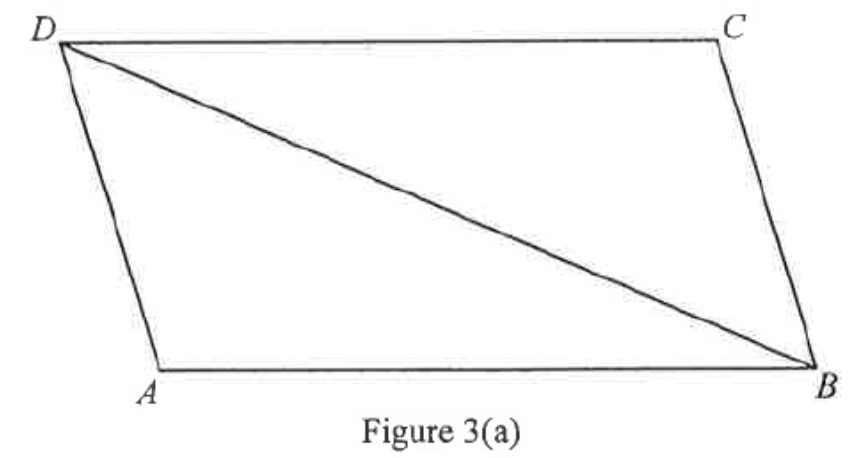
\includegraphics[width = .3\linewidth]{2018Figure1.3a}
		\end{figure}
		Find the length of $AD$. \\(2 marks)
		\item[(b)] The paper card in Figure 3(a) is folded along $BD$ such that the distance between $A$ and $C$ is 40 cm (see Figure 3(b)).
		\begin{figure}[H]
			\centering
			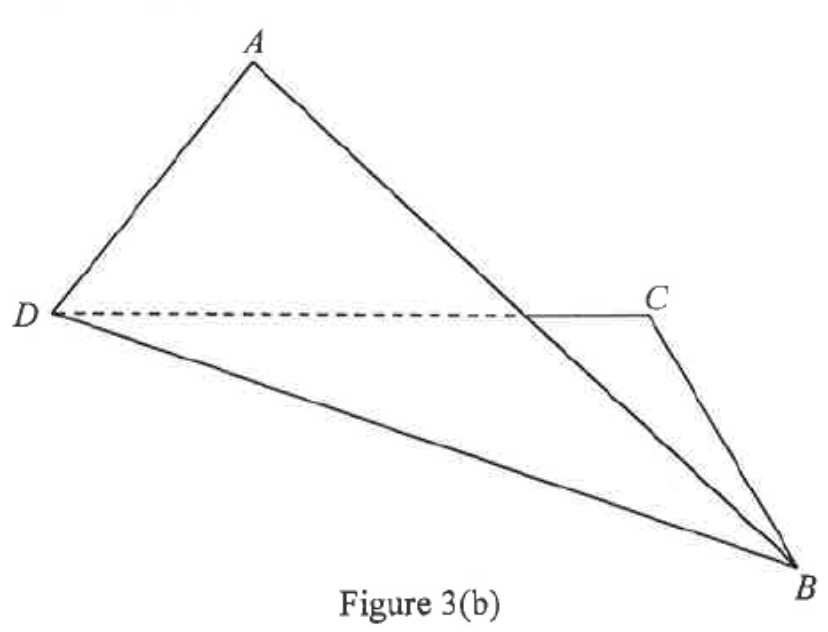
\includegraphics[width = .3\linewidth]{2018Figure1.3b}
		\end{figure}
		\begin{enumerate}
			\item[(i)] Find $\angle ABC$.
			\item[(ii)] Find the angle between the plane $ABD$ and the plane $BCD$.
		\end{enumerate}
		(5 marks)
	\end{enumerate}

	\item \textbf{HKDSE MATH CORE 2018 Past Paper I Q18}\\
	It is given that $f(x)$ partly varies as $x^2$ and partly varies as $x$. Suppose that $f(2) = 60$ and $f(3) = 99$.
	\begin{enumerate}
		\item[(a)] Find $f(x)$. \\(3 marks)
		\item[(b)] Let $Q$ be the vertex of the graph of $y = f(x)$ and $R$ be the vertex of $y = 27 - f(x)$.
		\begin{enumerate}
			\item[(i)] Using the method of completing the square, find the coordinates of $Q$.
			\item[(ii)] Write down the coordinates of $R$.
			\item[(iii)] The coordinates of the point $S$ are $(56, 0)$. Let $P$ be the circumcentre of $\triangle QRS$. Describe the geometric relationship between $P$, $Q$ and $R$. Explain your answer.
		\end{enumerate}
		(5 marks)
	\end{enumerate}

	\item \textbf{HKDSE MATH CORE 2018 Past Paper I Q19}\\
	The coordinates of the centre of the circle $C$ are $(8, 2)$. Denote the radius of $C$ by $r$. Let $L$ be the straight line $kx - 5y - 21 = 0$, where $k$ is a constant. It is given that $L$ is a tangent to $C$.
	\begin{enumerate}
		\item[(a)] Find the equation of $C$ in terms of $r$. Hence, express $r^2$ in terms of $k$. \\(4 marks)
		\item[(b)] $L$ passes through the point $D(18, 39)$.
		\begin{enumerate}
			\item[(i)] Find $r$.
			\item[(ii)] It is given that $L$ cuts the $y$-axis at the point $E$. Let $F$ be a point such that $C$ is the inscribed circle of $\triangle DEF$. Is $\triangle DEF$ an obtuse-angled triangle? Explain your answer.
		\end{enumerate}
		(8 marks)
	\end{enumerate}


\end{enumerate}
\end{document}